%% \documentclass[11pt]{article}
%%\usepackage{beamerarticle}
\documentclass[extsize,handout,10pt]{beamer}\usepackage[]{graphicx}\usepackage[]{color}
% maxwidth is the original width if it is less than linewidth
% otherwise use linewidth (to make sure the graphics do not exceed the margin)
\makeatletter
\def\maxwidth{ %
  \ifdim\Gin@nat@width>\linewidth
    \linewidth
  \else
    \Gin@nat@width
  \fi
}
\makeatother

\definecolor{fgcolor}{rgb}{0.251, 0.251, 0.251}
\newcommand{\hlnum}[1]{\textcolor[rgb]{0.502,0.086,1}{#1}}%
\newcommand{\hlstr}[1]{\textcolor[rgb]{1,0.4,0.2}{#1}}%
\newcommand{\hlcom}[1]{\textcolor[rgb]{1,0.251,0.502}{#1}}%
\newcommand{\hlopt}[1]{\textcolor[rgb]{0.251,0.251,0.251}{#1}}%
\newcommand{\hlstd}[1]{\textcolor[rgb]{0.251,0.251,0.251}{#1}}%
\newcommand{\hlkwa}[1]{\textcolor[rgb]{0.941,0.188,0.816}{#1}}%
\newcommand{\hlkwb}[1]{\textcolor[rgb]{0,0.439,0.902}{#1}}%
\newcommand{\hlkwc}[1]{\textcolor[rgb]{0.188,0.941,0.314}{#1}}%
\newcommand{\hlkwd}[1]{\textcolor[rgb]{0.69,0.188,0.941}{#1}}%
\let\hlipl\hlkwb

\usepackage{framed}
\makeatletter
\newenvironment{kframe}{%
 \def\at@end@of@kframe{}%
 \ifinner\ifhmode%
  \def\at@end@of@kframe{\end{minipage}}%
  \begin{minipage}{\columnwidth}%
 \fi\fi%
 \def\FrameCommand##1{\hskip\@totalleftmargin \hskip-\fboxsep
 \colorbox{shadecolor}{##1}\hskip-\fboxsep
     % There is no \\@totalrightmargin, so:
     \hskip-\linewidth \hskip-\@totalleftmargin \hskip\columnwidth}%
 \MakeFramed {\advance\hsize-\width
   \@totalleftmargin\z@ \linewidth\hsize
   \@setminipage}}%
 {\par\unskip\endMakeFramed%
 \at@end@of@kframe}
\makeatother

\definecolor{shadecolor}{rgb}{.97, .97, .97}
\definecolor{messagecolor}{rgb}{0, 0, 0}
\definecolor{warningcolor}{rgb}{1, 0, 1}
\definecolor{errorcolor}{rgb}{1, 0, 0}
\newenvironment{knitrout}{}{} % an empty environment to be redefined in TeX

\usepackage{alltt}
\usepackage{preambBeamer} %%preambBeamer for presentation (no hyperref, etc.)
\usepackage{texab} %%Abkürzungen

\mode<article>{\usepackage{}}
\mode<presentation>{\usetheme{} \usecolortheme{}}
\setbeamertemplate{footline}[frame number]





%\pgfpagesuselayout{4 on 1}[a4paper,border shrink=5mm, landscape]
\bibliographystyle{alpha}


\title{Introduction to the Generalized Linear Model}
\subtitle{Logistic and Poisson Regression}
\author{André Meichtry}
\institute{\GE \\ \ZHAWE}
\date{2020}
%\titlegraphic{\includegraphics[width=.2\textwidth]{/home/meichtry/BERATUNG/zhawD.jpg}}
\IfFileExists{upquote.sty}{\usepackage{upquote}}{}
\begin{document}

\selectlanguage{english}



\maketitle
%\frame{\tableofcontents}





\begin{frame}[fragile]
  \frametitle{Generalized Linear Model (GLM)}
\begin{itemize}
\item We want to generalize the linear model to discrete or continuous
  outcomes
\item Dichotomous event outcome, leading to \alert{Logistic regression}
\item Counts as outcome, leading to \alert{Poisson regression}
\end{itemize}
\begin{knitrout}\tiny
\definecolor{shadecolor}{rgb}{0.973, 0.973, 0.973}\color{fgcolor}

{\centering 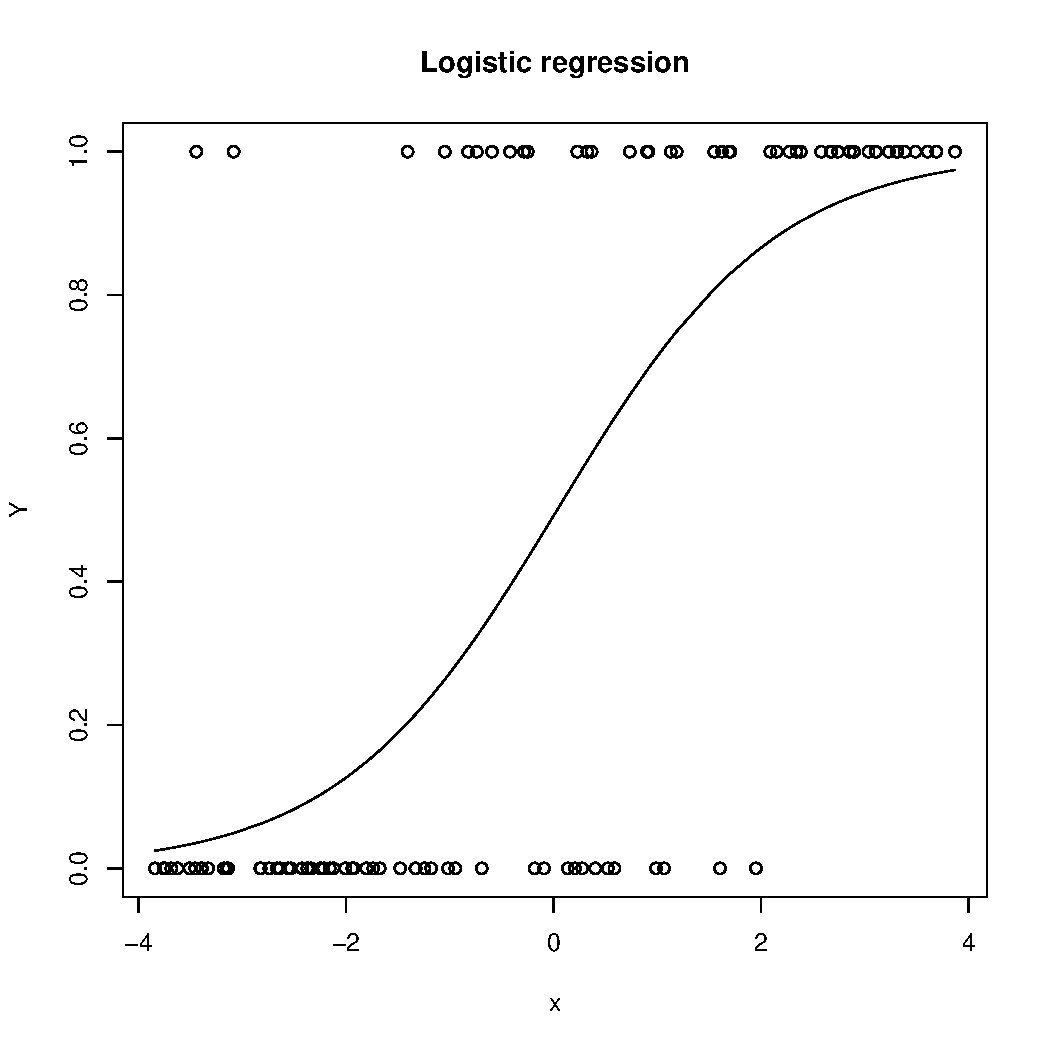
\includegraphics[width=.49\linewidth]{figures/GesWiss2unnamed-chunk-2-1} 

}



\end{knitrout}

\end{frame}


\begin{frame}
  \frametitle{Aspects of generalization}
  \begin{itemize}
  \item Link function
  \item Variance function
  \item Distribution of the exponential family
  \end{itemize}
\end{frame}

\begin{frame}
  \frametitle{Link function}
  \begin{itemize}
  \item \alert{Systematic part:} The expectation of the response,
    $\mu_i=\Erw(Y_i)$, is transformed with a \alert{link function}.
  \item This quantity is a linear function of the parameter $\beta_j$,
    called the \alert{linear predictor} $\eta_i$ with the link function
    $h(\cdot)$
    \begin{equation}
      \label{eq:55}
      \boxed{h(\Erw(Y_i))=h(\mu_i)=\eta_i=\bmath{x}^T_i\bmath{\beta}.}
    \end{equation}
  \end{itemize}
\begin{itemize}
\item Usual Link functions
\begin{itemize}
  \item Linear regression: Identity function
  \item Logistic regression: logit function
  \item Poisson regression: log function
  \end{itemize}
  \end{itemize}
\end{frame}



\begin{frame}
  \frametitle{Variance function}
  \begin{itemize}
  \item \alert{Random part:} The variance $\Var(Y_i)$ is a function of
    the expectation,
    \begin{equation}
      \label{eq:56}
      \boxed{\Var(Y_i)=\phi v(\mu_i),}
    \end{equation}
    where $v(\cdot)$ is the \alert{variance function} and $\phi$ is the
    \alert{dispersion parameter}, which has to be estimated or not.
  \end{itemize}
\begin{itemize}
\item Usual variance functions
\begin{itemize}
  \item Linear regression: $v(\mu_i)=1$ with $\phi=\sigma^2$
  \item Logistic regression: $v(\mu_i)=\mu_i(1-\mu_i)$ and $\phi=1$
  \item Poisson regression: $v(\mu_i)=\mu_i$ and $\phi=1$
  \end{itemize}
  \end{itemize}
\end{frame}



\begin{frame}
  \frametitle{Distributions}
  \begin{itemize}
  \item Each class of a GLM follow a model with density of the
    \alert{exponential family}\footnote{\tiny distributions of the
      exponential family have densities 
      $f(y_i)=\exp\{(y_i\theta_{i}-A(\theta_i))/\phi+B(y_i,\phi)\}$
      with $\theta_{i}$ as the \alert{canonical parameter} with ca be
      expressed trough $\mu_i$. One can show that
      $\Erw(Y_i)=\mu_i=A'(\theta_{i})$ and
      $\Var(Y_i)=A''(\theta_i)\phi$. The function $A(\cdot)$ fixes the
      exponential family, $B(\cdot)$ is a normalizing function.}. Special cases and most often used are:
    \item The \alert{Normal distribution}
    \item The \alert{Binomial distribution}
    \item The \alert{Poisson distribution}
  \end{itemize}

\end{frame}


\begin{frame}
  \frametitle{Recap: Linear Model}
  \begin{itemize}
  \item $Y_i\sim \N(\bmath{x}^T_i\bmath{\beta},\sigma^2)$.
  \item The model can be written:
    $Y_i=\bmath{x}^T_i\bmath{\beta}+\epsilon_i$. 
  \item The expectation
    $\mu_i$ is
    \begin{equation}
      \label{eq:54}
      \mu_i=\Erw(Y_i)=\bmath{x}^T_i\bmath{\beta}.
    \end{equation}
  \item The link function $h(\cdot)$ is the identity and the
    variance function is $v(\mu_i)=1$, the dispersion parameter is
    known, $\phi=\sigma^2$.
  \item Interpretation: $\beta_j$ is the difference in expectations
    for two subpopulations that differ on $x_j$ by on unit (slope).
  \end{itemize}
\end{frame}




\begin{frame}[fragile]
  \frametitle{Recap: Linear Model for Fertility}
  \begin{itemize}
  \item Estimation with least squares:  \texttt{lm()} 
  \end{itemize}

\begin{knitrout}\tiny
\definecolor{shadecolor}{rgb}{0.973, 0.973, 0.973}\color{fgcolor}\begin{kframe}
\begin{alltt}
\hlstd{modlm}\hlkwb{<-}\hlkwd{lm}\hlstd{(Fertility}\hlopt{~}\hlstd{.,swiss)}
\hlstd{modlm0}\hlkwb{<-}\hlkwd{lm}\hlstd{(Fertility}\hlopt{~}\hlnum{1}\hlstd{,swiss)} \hlcom{##for later}
\hlkwd{summary}\hlstd{(modlm)}
\end{alltt}
\begin{verbatim}
## 
## Call:
## lm(formula = Fertility ~ ., data = swiss)
## 
## Residuals:
##      Min       1Q   Median       3Q      Max 
## -15.2743  -5.2617   0.5032   4.1198  15.3213 
## 
## Coefficients:
##                  Estimate Std. Error t value    Pr(>|t|)
## (Intercept)      66.91518   10.70604   6.250 0.000000191
## Agriculture      -0.17211    0.07030  -2.448     0.01873
## Examination      -0.25801    0.25388  -1.016     0.31546
## Education        -0.87094    0.18303  -4.758 0.000024306
## Catholic          0.10412    0.03526   2.953     0.00519
## Infant.Mortality  1.07705    0.38172   2.822     0.00734
## 
## Residual standard error: 7.165 on 41 degrees of freedom
## Multiple R-squared:  0.7067,	Adjusted R-squared:  0.671 
## F-statistic: 19.76 on 5 and 41 DF,  p-value: 0.0000000005594
\end{verbatim}
\end{kframe}
\end{knitrout}
\end{frame}




\begin{frame}[fragile]
  \frametitle{The same model as GLM}

    \begin{itemize}
    \item Estimation with maximum likelihood: \texttt{glm()}
    \end{itemize}

\begin{knitrout}\tiny
\definecolor{shadecolor}{rgb}{0.973, 0.973, 0.973}\color{fgcolor}\begin{kframe}
\begin{alltt}
\hlstd{modglm}\hlkwb{<-}\hlkwd{glm}\hlstd{(Fertility}\hlopt{~}\hlstd{.,swiss,}\hlkwc{family}\hlstd{=gaussian)}
\hlstd{modglm0}\hlkwb{<-}\hlkwd{glm}\hlstd{(Fertility}\hlopt{~}\hlnum{1}\hlstd{,swiss,}\hlkwc{family}\hlstd{=gaussian)}\hlcom{## for later}
\hlkwd{summary}\hlstd{(modglm)}
\end{alltt}
\begin{verbatim}
## 
## Call:
## glm(formula = Fertility ~ ., family = gaussian, data = swiss)
## 
## Deviance Residuals: 
##      Min        1Q    Median        3Q       Max  
## -15.2743   -5.2617    0.5032    4.1198   15.3213  
## 
## Coefficients:
##                  Estimate Std. Error t value    Pr(>|t|)
## (Intercept)      66.91518   10.70604   6.250 0.000000191
## Agriculture      -0.17211    0.07030  -2.448     0.01873
## Examination      -0.25801    0.25388  -1.016     0.31546
## Education        -0.87094    0.18303  -4.758 0.000024306
## Catholic          0.10412    0.03526   2.953     0.00519
## Infant.Mortality  1.07705    0.38172   2.822     0.00734
## 
## (Dispersion parameter for gaussian family taken to be 51.34251)
## 
##     Null deviance: 7178  on 46  degrees of freedom
## Residual deviance: 2105  on 41  degrees of freedom
## AIC: 326.07
## 
## Number of Fisher Scoring iterations: 2
\end{verbatim}
\end{kframe}
\end{knitrout}
\end{frame}

\begin{frame}[fragile]
  \frametitle{What is different?}


    \begin{itemize}
    \item ``Deviance'' versus Sum of Squares
    \item ``Likelihood ratio tests'' versus $F$-tests
    \item Explanations in next slides
    \end{itemize}

\begin{knitrout}\tiny
\definecolor{shadecolor}{rgb}{0.973, 0.973, 0.973}\color{fgcolor}\begin{kframe}
\begin{alltt}
\hlkwd{anova}\hlstd{(modglm,modglm0,}\hlkwc{test}\hlstd{=}\hlstr{"LR"}\hlstd{)}
\end{alltt}
\begin{verbatim}
## Analysis of Deviance Table
## 
## Model 1: Fertility ~ Agriculture + Examination + Education + Catholic + 
##     Infant.Mortality
## Model 2: Fertility ~ 1
##   Resid. Df Resid. Dev Df Deviance              Pr(>Chi)
## 1        41       2105                                  
## 2        46       7178 -5  -5072.9 < 0.00000000000000022
\end{verbatim}
\begin{alltt}
\hlkwd{anova}\hlstd{(modlm,modlm0,}\hlkwc{test}\hlstd{=}\hlstr{"F"}\hlstd{)}
\end{alltt}
\begin{verbatim}
## Analysis of Variance Table
## 
## Model 1: Fertility ~ Agriculture + Examination + Education + Catholic + 
##     Infant.Mortality
## Model 2: Fertility ~ 1
##   Res.Df  RSS Df Sum of Sq      F          Pr(>F)
## 1     41 2105                                    
## 2     46 7178 -5   -5072.9 19.761 0.0000000005594
\end{verbatim}
\end{kframe}
\end{knitrout}
\end{frame}




\begin{frame}
  \frametitle{Estimation and Tests}
  \begin{itemize}
  \item Estimation via \alert{Maximum Likelihood Principle} 
  \item We look at the (logarithmic) probability of the data \alert{as function of the
    parameters} and search the maximum.
  \item The log-likelihood $l$ is
    \begin{equation}
      \label{eq:1}
      l(\bmath{\beta})=\sum_{i=1}^n \log \Pr(Y_i=y_i \mid \bmath{x}_i,\bmath{\beta})
    \end{equation}
  \item The $\bmath{\beta}$ that maximizes $l(\bmath{\beta})$ is called the
    \alert{Maximum Likelihood Estimate (MLE)} $\hat{\bmath{\beta}}$
  \item One can show that the MLE has an asymptotic normal
    distribution.
  \end{itemize}
\end{frame}



\begin{frame}
  \frametitle{Estimation and Tests}
  \begin{itemize}
  \item \alert{Residual Deviance} replaces the \alert{residual sum of squares} 
    and is defined as
    \begin{equation}
      \label{eq:2}
      D=2(l_{max}-l(\hat{\bmath{\beta}}))
    \end{equation}
  \item $l_{max}$ is the likelihood for the ``maximal'', the saturated
    model (one parameter for each observation $i$)
  \item \alert{Null Deviance} replaces the \alert{total sum of
      squares}
\begin{equation}
      \label{eq:2}
      D=2(l_{max}-l_0)
    \end{equation}
\end{itemize}
\end{frame}




\begin{frame}
  \frametitle{Estimation and Tests}
  \begin{itemize}
  \item \alert{Likelihood-Ratio-Test:} The difference in deviance 
    \begin{equation}
      \label{eq:3}
      2(l_{Large}-l_{Small})
    \end{equation}
  \item has an asymptotic chi-square distribution 
  \item with the difference of the number of parameters as degrees of
    freedom.
\end{itemize}
\begin{alertblock}

\begin{itemize}
\item $H_0$: Modell small with $p_{Small}$ parameters is true.
\item $H_1$: Modell large with $p_{Large}>p_{Small}$ parameters is
  true.
\item $2(l_{Large}-l_{Small})\overset{approx}{\sim} \chi^2_{p_{Large}-p_{Small}}$
\end{itemize}
\end{alertblock}

\end{frame}


\begin{frame}
  \frametitle{Logistic regression}
  \begin{itemize}
  \item The distribution of the $Y_i$ is binomial,
    $$Y_i\sim \Bin{\mu_i=\pi_i,n=1}$$
  \item The model for $\mu_i=\pi_i$ can be written
    \begin{equation}
      \label{eq:57}
      \logit(\pi_i)=\bmath{x}^T_i\bmath{\beta},
    \end{equation}
  \item The link function is
    $h(\pi_i)=\logit(\pi_i)=\log(\pi_i/(1-\pi_i))=\log \mathrm{odds}$
  \item The variance function $v(\pi)=\pi(1-\pi)$ and $\phi=1$.
  \item Interpretation: $\beta_j$ (except for the intercept) is the difference in logits (\alert{log
    odds ratio}) for two subpopulations that differ on $x_j$ by on unit.
  \item $\exp(\beta_j)$ (except for the intercept) is the \alert{odds
      ratio} $OR$ for the event for two subpopulations that differ on $x_j$ by one
    unit.
  \end{itemize}
\end{frame}


\begin{frame}[fragile]
  \frametitle{Example with one continuous predictor}

  \begin{itemize}
  \item Simulate some data:
  \end{itemize}

\begin{knitrout}\tiny
\definecolor{shadecolor}{rgb}{0.973, 0.973, 0.973}\color{fgcolor}\begin{kframe}
\begin{alltt}
\hlkwd{set.seed}\hlstd{(}\hlnum{10}\hlstd{)}
\hlcom{##Sample Size}
\hlstd{N}\hlkwb{<-}\hlnum{30}
\hlcom{##predictor}
\hlstd{x}\hlkwb{<-}\hlkwd{sort}\hlstd{(}\hlkwd{runif}\hlstd{(N,}\hlopt{-}\hlnum{5}\hlstd{,}\hlnum{5}\hlstd{))}
\hlcom{##parameters}
\hlstd{alpha}\hlkwb{<-}\hlnum{0}
\hlstd{beta}\hlkwb{<-}\hlnum{1}
\hlcom{##linear predictor}
\hlstd{eta}\hlkwb{<-}\hlstd{alpha}\hlopt{+}\hlstd{x}\hlopt{*}\hlstd{beta}
\hlcom{##linear predictor logit E(Y) = eta}
\hlcom{##Inverse function of the logit function is the logistic function,}
\hlcom{##logistic(eta)=E(Y)=mu (here mu is a probability, often written pi)}
\hlstd{pi}\hlkwb{<-}\hlkwd{exp}\hlstd{(eta)}\hlopt{/}\hlstd{(}\hlnum{1}\hlopt{+}\hlkwd{exp}\hlstd{(eta))}
\hlcom{##Draw N from binomial distribution with parameters pi and 1}
\hlstd{Y}\hlkwb{<-}\hlkwd{rbinom}\hlstd{(N,}\hlkwc{size}\hlstd{=}\hlnum{1}\hlstd{,}\hlkwc{prob}\hlstd{=pi)}
\end{alltt}
\end{kframe}
\end{knitrout}

\end{frame}


\begin{frame}[fragile]
  \frametitle{Example with one continuous predictor}

\begin{knitrout}\tiny
\definecolor{shadecolor}{rgb}{0.973, 0.973, 0.973}\color{fgcolor}\begin{kframe}
\begin{alltt}
\hlkwd{headTail}\hlstd{(}\hlkwd{cbind}\hlstd{(x,Y))}
\end{alltt}
\begin{verbatim}
##         x   Y
## 1   -4.48   0
## 2   -4.15   0
## 3   -3.86   0
## 4   -2.75   0
## ...   ... ...
## 27   2.75   1
## 28   3.36   1
## 29   3.38   1
## 30   3.65   1
\end{verbatim}
\end{kframe}
\end{knitrout}


\begin{knitrout}\tiny
\definecolor{shadecolor}{rgb}{0.973, 0.973, 0.973}\color{fgcolor}\begin{kframe}
\begin{alltt}
\hlstd{mod0}\hlkwb{<-}\hlkwd{glm}\hlstd{(Y}\hlopt{~}\hlnum{1}\hlstd{,}\hlkwc{family}\hlstd{=}\hlstr{"binomial"}\hlstd{)}
\hlstd{mod}\hlkwb{<-}\hlkwd{glm}\hlstd{(Y}\hlopt{~}\hlstd{x,}\hlkwc{family}\hlstd{=}\hlstr{"binomial"}\hlstd{)}
\hlkwd{summary}\hlstd{(mod)}
\end{alltt}
\begin{verbatim}
## 
## Call:
## glm(formula = Y ~ x, family = "binomial")
## 
## Deviance Residuals: 
##     Min       1Q   Median       3Q      Max  
## -1.6720  -0.5881  -0.1558   0.4501   2.2860  
## 
## Coefficients:
##             Estimate Std. Error z value Pr(>|z|)
## (Intercept)  -0.1250     0.5440  -0.230  0.81826
## x             1.0696     0.3597   2.974  0.00294
## 
## (Dispersion parameter for binomial family taken to be 1)
## 
##     Null deviance: 41.054  on 29  degrees of freedom
## Residual deviance: 21.906  on 28  degrees of freedom
## AIC: 25.906
## 
## Number of Fisher Scoring iterations: 5
\end{verbatim}
\end{kframe}
\end{knitrout}

\end{frame}



\begin{frame}[fragile]
  \frametitle{Wald-tests and LRT-Tests}

  \begin{itemize}
  \item Tests of individual coefficients based on approximative normality are
    called \alert{Wald}-tests. 
  \item Crude assumption about the
    shape of the likelihood. 
  \item The LRT takes the likelihood values as they are. 
  \item Therefore LR-tests are usually superior to Wald-tests
  \item They are asymptotically equivalent.
  \item \texttt{confint()} constructs LR confidence intervals if a
    glm-object is given as argument.
  \end{itemize}

\begin{knitrout}\tiny
\definecolor{shadecolor}{rgb}{0.973, 0.973, 0.973}\color{fgcolor}\begin{kframe}
\begin{alltt}
\hlkwd{anova}\hlstd{(mod,mod0,}\hlkwc{test}\hlstd{=}\hlstr{"LR"}\hlstd{)}
\end{alltt}
\begin{verbatim}
## Analysis of Deviance Table
## 
## Model 1: Y ~ x
## Model 2: Y ~ 1
##   Resid. Df Resid. Dev Df Deviance  Pr(>Chi)
## 1        28     21.906                      
## 2        29     41.054 -1  -19.148 0.0000121
\end{verbatim}
\begin{alltt}
\hlkwd{confint}\hlstd{(mod)}
\end{alltt}


{\ttfamily\noindent\itshape\color{messagecolor}{\#\# Waiting for profiling to be done...}}\begin{verbatim}
##                  2.5 %    97.5 %
## (Intercept) -1.2351381 0.9959719
## x            0.4936061 1.9548316
\end{verbatim}
\end{kframe}
\end{knitrout}




\end{frame}


\begin{frame}[fragile]
  \frametitle{Model and data} 

\begin{knitrout}\tiny
\definecolor{shadecolor}{rgb}{0.973, 0.973, 0.973}\color{fgcolor}\begin{kframe}
\begin{alltt}
\hlstd{pred}\hlkwb{<-}\hlkwd{predict}\hlstd{(mod,}\hlkwc{type}\hlstd{=}\hlstr{"response"}\hlstd{)}
\hlkwd{plot}\hlstd{(x,Y)}
\hlkwd{lines}\hlstd{(x,pred)}
\end{alltt}
\end{kframe}

{\centering 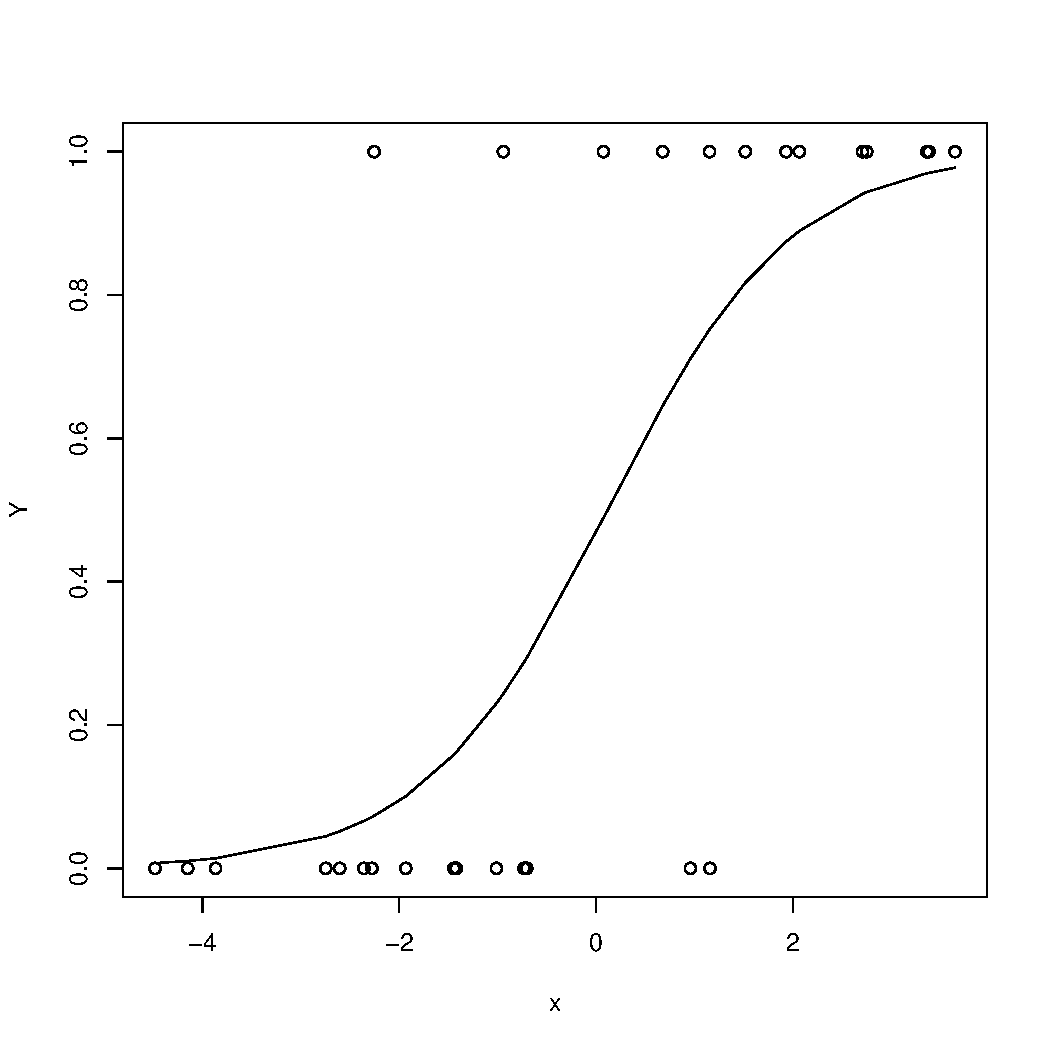
\includegraphics[width=.49\linewidth]{figures/GesWiss2unnamed-chunk-11-1} 

}



\end{knitrout}
 

\end{frame}




\begin{frame}[fragile]
  \frametitle{Residual analysis} 
What residuals are is not unambiguous:
  \begin{itemize}
  \item Raw residuals (Response residuals) $R_i=Y_i-\hat{\pi_i}$
  \item Working residuals (transformed on the space of the linear predictor)
  \item Deviance residuals: $\sign(Y_i-\hat{\pi_i})\cdot\sqrt{d_i}$ with
    $d_i$ as the contribution $i$ to the deviance\footnote{would be equal to the square root of
    a squared residual in normal distribution.}.
  \item Pearson residuals (Raw residuals divided by the standard
    deviation)
  \end{itemize}
 

\end{frame}



\begin{frame}[fragile]
  \frametitle{Residual analysis} 

  \begin{itemize}
  \item Working residuals against linear predictor
  \item Response residuals against fitted values
  \end{itemize}

\begin{knitrout}\tiny
\definecolor{shadecolor}{rgb}{0.973, 0.973, 0.973}\color{fgcolor}\begin{kframe}
\begin{alltt}
\hlkwd{plot}\hlstd{(mod,}\hlkwc{which}\hlstd{=}\hlnum{1}\hlstd{)}
\end{alltt}
\end{kframe}

{\centering 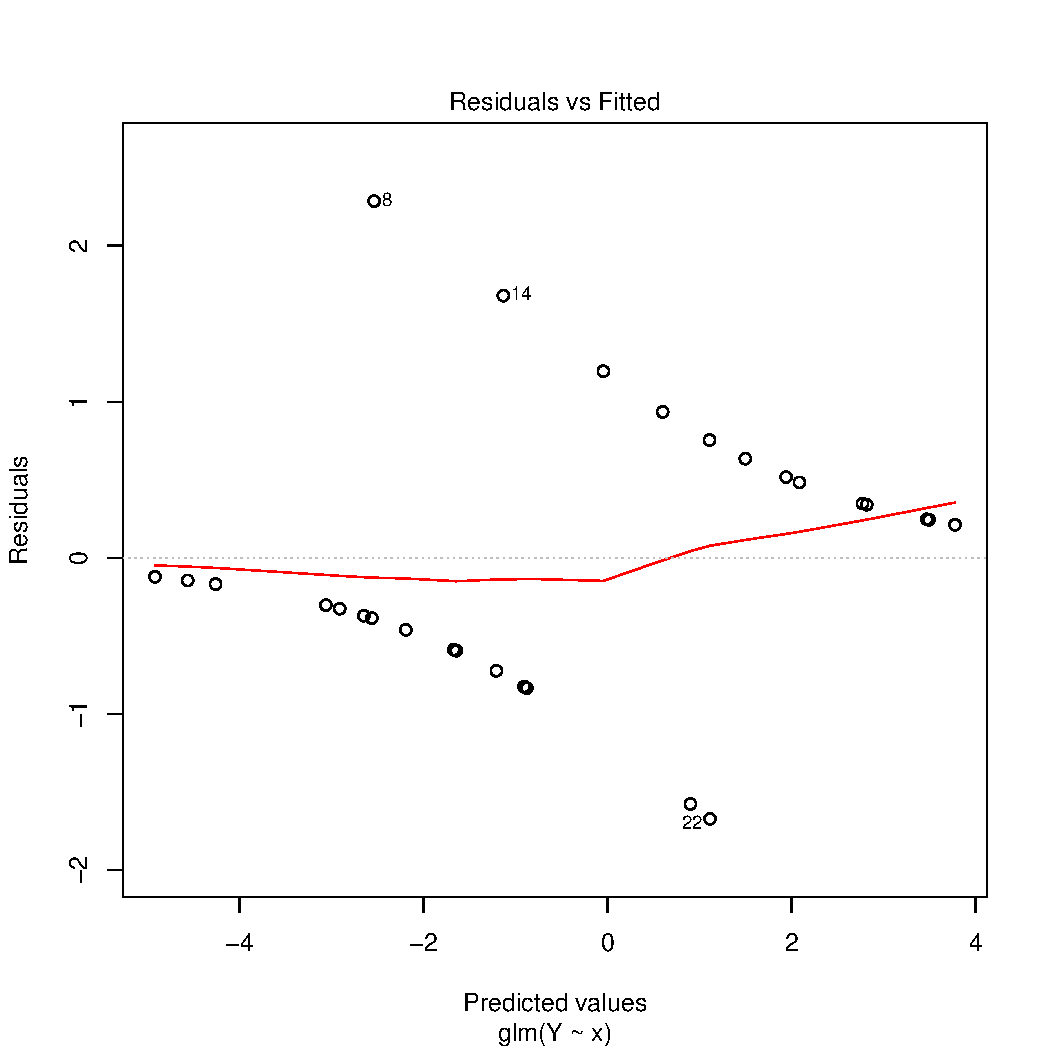
\includegraphics[width=.49\linewidth]{figures/GesWiss2unnamed-chunk-12-1} 

}



\end{knitrout}
 

\end{frame}




\begin{frame}[fragile]
  \frametitle{Example 2: HIV} 
\begin{knitrout}\tiny
\definecolor{shadecolor}{rgb}{0.973, 0.973, 0.973}\color{fgcolor}\begin{kframe}
\begin{alltt}
\hlstd{d.hiv}\hlkwb{<-}\hlkwd{read.csv}\hlstd{(}\hlstr{"https://raw.githubusercontent.com/mcdr65/PhDCareRehab/master/Data/HIV.csv"}\hlstd{)}
\hlcom{#str(d.hiv)}
\hlstd{f}\hlkwb{<-}\hlnum{1}\hlopt{:}\hlnum{11}
\hlstd{d.hiv[,f]}\hlkwb{<-}\hlkwd{lapply}\hlstd{(d.hiv[,f],as.factor)}
\end{alltt}
\end{kframe}
\end{knitrout}

\begin{knitrout}\tiny
\definecolor{shadecolor}{rgb}{0.973, 0.973, 0.973}\color{fgcolor}\begin{kframe}
\begin{alltt}
\hlkwd{head}\hlstd{(d.hiv)}
\end{alltt}
\begin{verbatim}
##    id age3 gender race3 educ4 employment disability dep anxpoms8 paindic aids
## 1 201    1      1     4     3          0          0   0     <NA>       1    1
## 2 202    1      1     2     4          0          1   0        0       1    0
## 3 204    2      1     5     4          1          0   1        1       1    0
## 4 205    1      1     5     3          1          0   0        1       0    0
## 5 206    3      1     5     1          0          1   1        1       1    1
## 6 207    1      2     4     4          0          1   1        0       1    1
\end{verbatim}
\begin{alltt}
\hlkwd{summary}\hlstd{(d.hiv)}
\end{alltt}
\begin{verbatim}
##        id      age3    gender  race3   educ4   employment disability dep     anxpoms8   paindic    aids   
##  201    :  1   1: 86   1:216   2:122   1: 47   0:267      0   : 80   0:159   0   :163   0   :141   0:151  
##  202    :  1   2:133   2: 77   4:129   2: 94   1: 49      1   :235   1:157   1   :145   1   :174   1:165  
##  204    :  1   3: 97   3: 23   5: 65   3:107              NA's:  1           NA's:  8   NA's:  1          
##  205    :  1                           4: 68                                                              
##  206    :  1                                                                                              
##  207    :  1                                                                                              
##  (Other):310
\end{verbatim}
\end{kframe}
\end{knitrout}
 

\end{frame}



\begin{frame}[fragile]
  \frametitle{Example 2: Marginal Wald tests} 



\begin{knitrout}\tiny
\definecolor{shadecolor}{rgb}{0.973, 0.973, 0.973}\color{fgcolor}\begin{kframe}
\begin{alltt}
\hlstd{fit} \hlkwb{<-} \hlkwd{glm}\hlstd{(aids}\hlopt{~}\hlstd{age3}\hlopt{+}\hlstd{gender}\hlopt{+}\hlstd{race3}\hlopt{+}\hlstd{educ4}\hlopt{+}\hlstd{employment}\hlopt{+}\hlstd{disability}\hlopt{+}\hlstd{dep}\hlopt{+}\hlstd{paindic,} \hlkwc{family}\hlstd{=}\hlstr{"binomial"}\hlstd{,}\hlkwc{data}\hlstd{=d.hiv)}
\hlkwd{summary}\hlstd{(fit)}
\end{alltt}
\begin{verbatim}
## 
## Call:
## glm(formula = aids ~ age3 + gender + race3 + educ4 + employment + 
##     disability + dep + paindic, family = "binomial", data = d.hiv)
## 
## Deviance Residuals: 
##    Min      1Q  Median      3Q     Max  
## -1.816  -1.095   0.652   1.008   2.063  
## 
## Coefficients:
##              Estimate Std. Error z value Pr(>|z|)
## (Intercept) -0.960436   0.570402  -1.684   0.0922
## age32        0.191440   0.299411   0.639   0.5226
## age33        0.004589   0.325009   0.014   0.9887
## gender2     -0.253102   0.306745  -0.825   0.4093
## gender3     -0.603355   0.500796  -1.205   0.2283
## race34       0.560104   0.296623   1.888   0.0590
## race35       0.380728   0.338857   1.124   0.2612
## educ42      -0.127337   0.400751  -0.318   0.7507
## educ43       0.515187   0.393228   1.310   0.1901
## educ44      -0.010437   0.436651  -0.024   0.9809
## employment1 -0.210049   0.501418  -0.419   0.6753
## disability1  0.909227   0.406726   2.235   0.0254
## dep1        -0.451316   0.256693  -1.758   0.0787
## paindic1     0.411642   0.256803   1.603   0.1089
## 
## (Dispersion parameter for binomial family taken to be 1)
## 
##     Null deviance: 434.48  on 313  degrees of freedom
## Residual deviance: 399.67  on 300  degrees of freedom
##   (2 observations deleted due to missingness)
## AIC: 427.67
## 
## Number of Fisher Scoring iterations: 4
\end{verbatim}
\end{kframe}
\end{knitrout}


\end{frame}




\begin{frame}[fragile]
  \frametitle{Example 2: Sequential LR tests} 

\begin{knitrout}\tiny
\definecolor{shadecolor}{rgb}{0.973, 0.973, 0.973}\color{fgcolor}\begin{kframe}
\begin{alltt}
\hlkwd{anova}\hlstd{(fit,}\hlkwc{test}\hlstd{=}\hlstr{"LR"}\hlstd{)}
\end{alltt}
\begin{verbatim}
## Analysis of Deviance Table
## 
## Model: binomial, link: logit
## 
## Response: aids
## 
## Terms added sequentially (first to last)
## 
## 
##            Df Deviance Resid. Df Resid. Dev Pr(>Chi)
## NULL                         313     434.48         
## age3        2   0.9382       311     433.54 0.625560
## gender      2   4.5941       309     428.95 0.100553
## race3       2   3.3381       307     425.61 0.188425
## educ4       3   7.0244       304     418.59 0.071125
## employment  1   9.6518       303     408.93 0.001892
## disability  1   4.7482       302     404.19 0.029330
## dep         1   1.9338       301     402.25 0.164346
## paindic     1   2.5849       300     399.67 0.107885
\end{verbatim}
\end{kframe}
\end{knitrout}
 
\begin{itemize}
\item One could proceed with different model comparisons.
\end{itemize}

\end{frame}






\begin{frame}[fragile]
  \frametitle{Example 2: Tukey-Anscombe Plot} 

\begin{knitrout}\tiny
\definecolor{shadecolor}{rgb}{0.973, 0.973, 0.973}\color{fgcolor}\begin{kframe}
\begin{alltt}
\hlkwd{plot}\hlstd{(fit,}\hlkwc{which}\hlstd{=}\hlnum{1}\hlstd{)}
\end{alltt}
\end{kframe}

{\centering 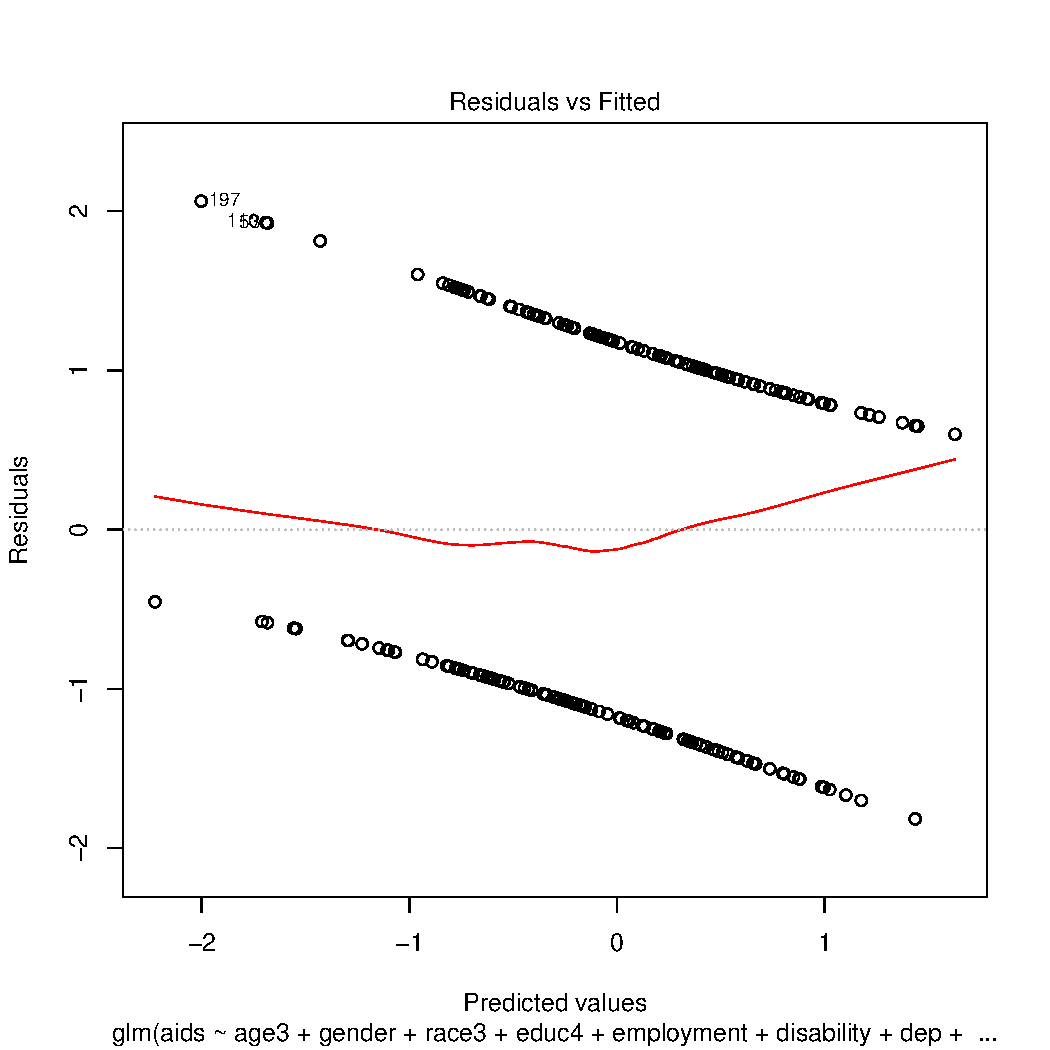
\includegraphics[width=.49\linewidth]{figures/GesWiss2unnamed-chunk-17-1} 

}



\end{knitrout}
 

\end{frame}



















\begin{frame}
  \frametitle{Poisson regression}
  \begin{itemize}
  \item Model for counts $Y_i$
  \item The distribution of the $Y_i$ is Poisson, $Y_i \sim \Pois{\mu_i}$ with expectation $\mu_i$.
  \item The model is
  \begin{equation}
  \label{eq:4}
  \log(\mu_i)=\bmath{x}^T_i\bmath{\beta}
  \end{equation}
  \item The link function is $h(\mu_i)=\log(\mu_i)$
                                            \item The variance
  function is $v(\mu_i)=\mu_i$ und $\phi=1$.
  \item $\beta_j$ is the difference in the logs of expected counts 
  \item $\exp(\beta_j)$ is the (risk, rate, count) ratio for two
  subpopulations that differ on $x_j$ by on unit (except for the
                                                  intercept.)
\end{itemize}
\end{frame}


\end{document}


%%% Local Variables:
%%% mode: latex
%%% TeX-master: t
%%% End:
